\newpage		
\section*{Лист 3}
	\subsection*{Задача 1}
	\noindent
	Заметим что идеальный треугольник определяется 3 своими вершинами, лежащими на абсолюте, а следовательно если треугольник перешел сам в себя, то и его вершины перешли сами в себя и наоборот. Следовательно группа симметрий идеального треугольника изоморфна $S_{3}$.
	
	\subsection*{Задача 2}
	\begin{figure}[h!]
		\center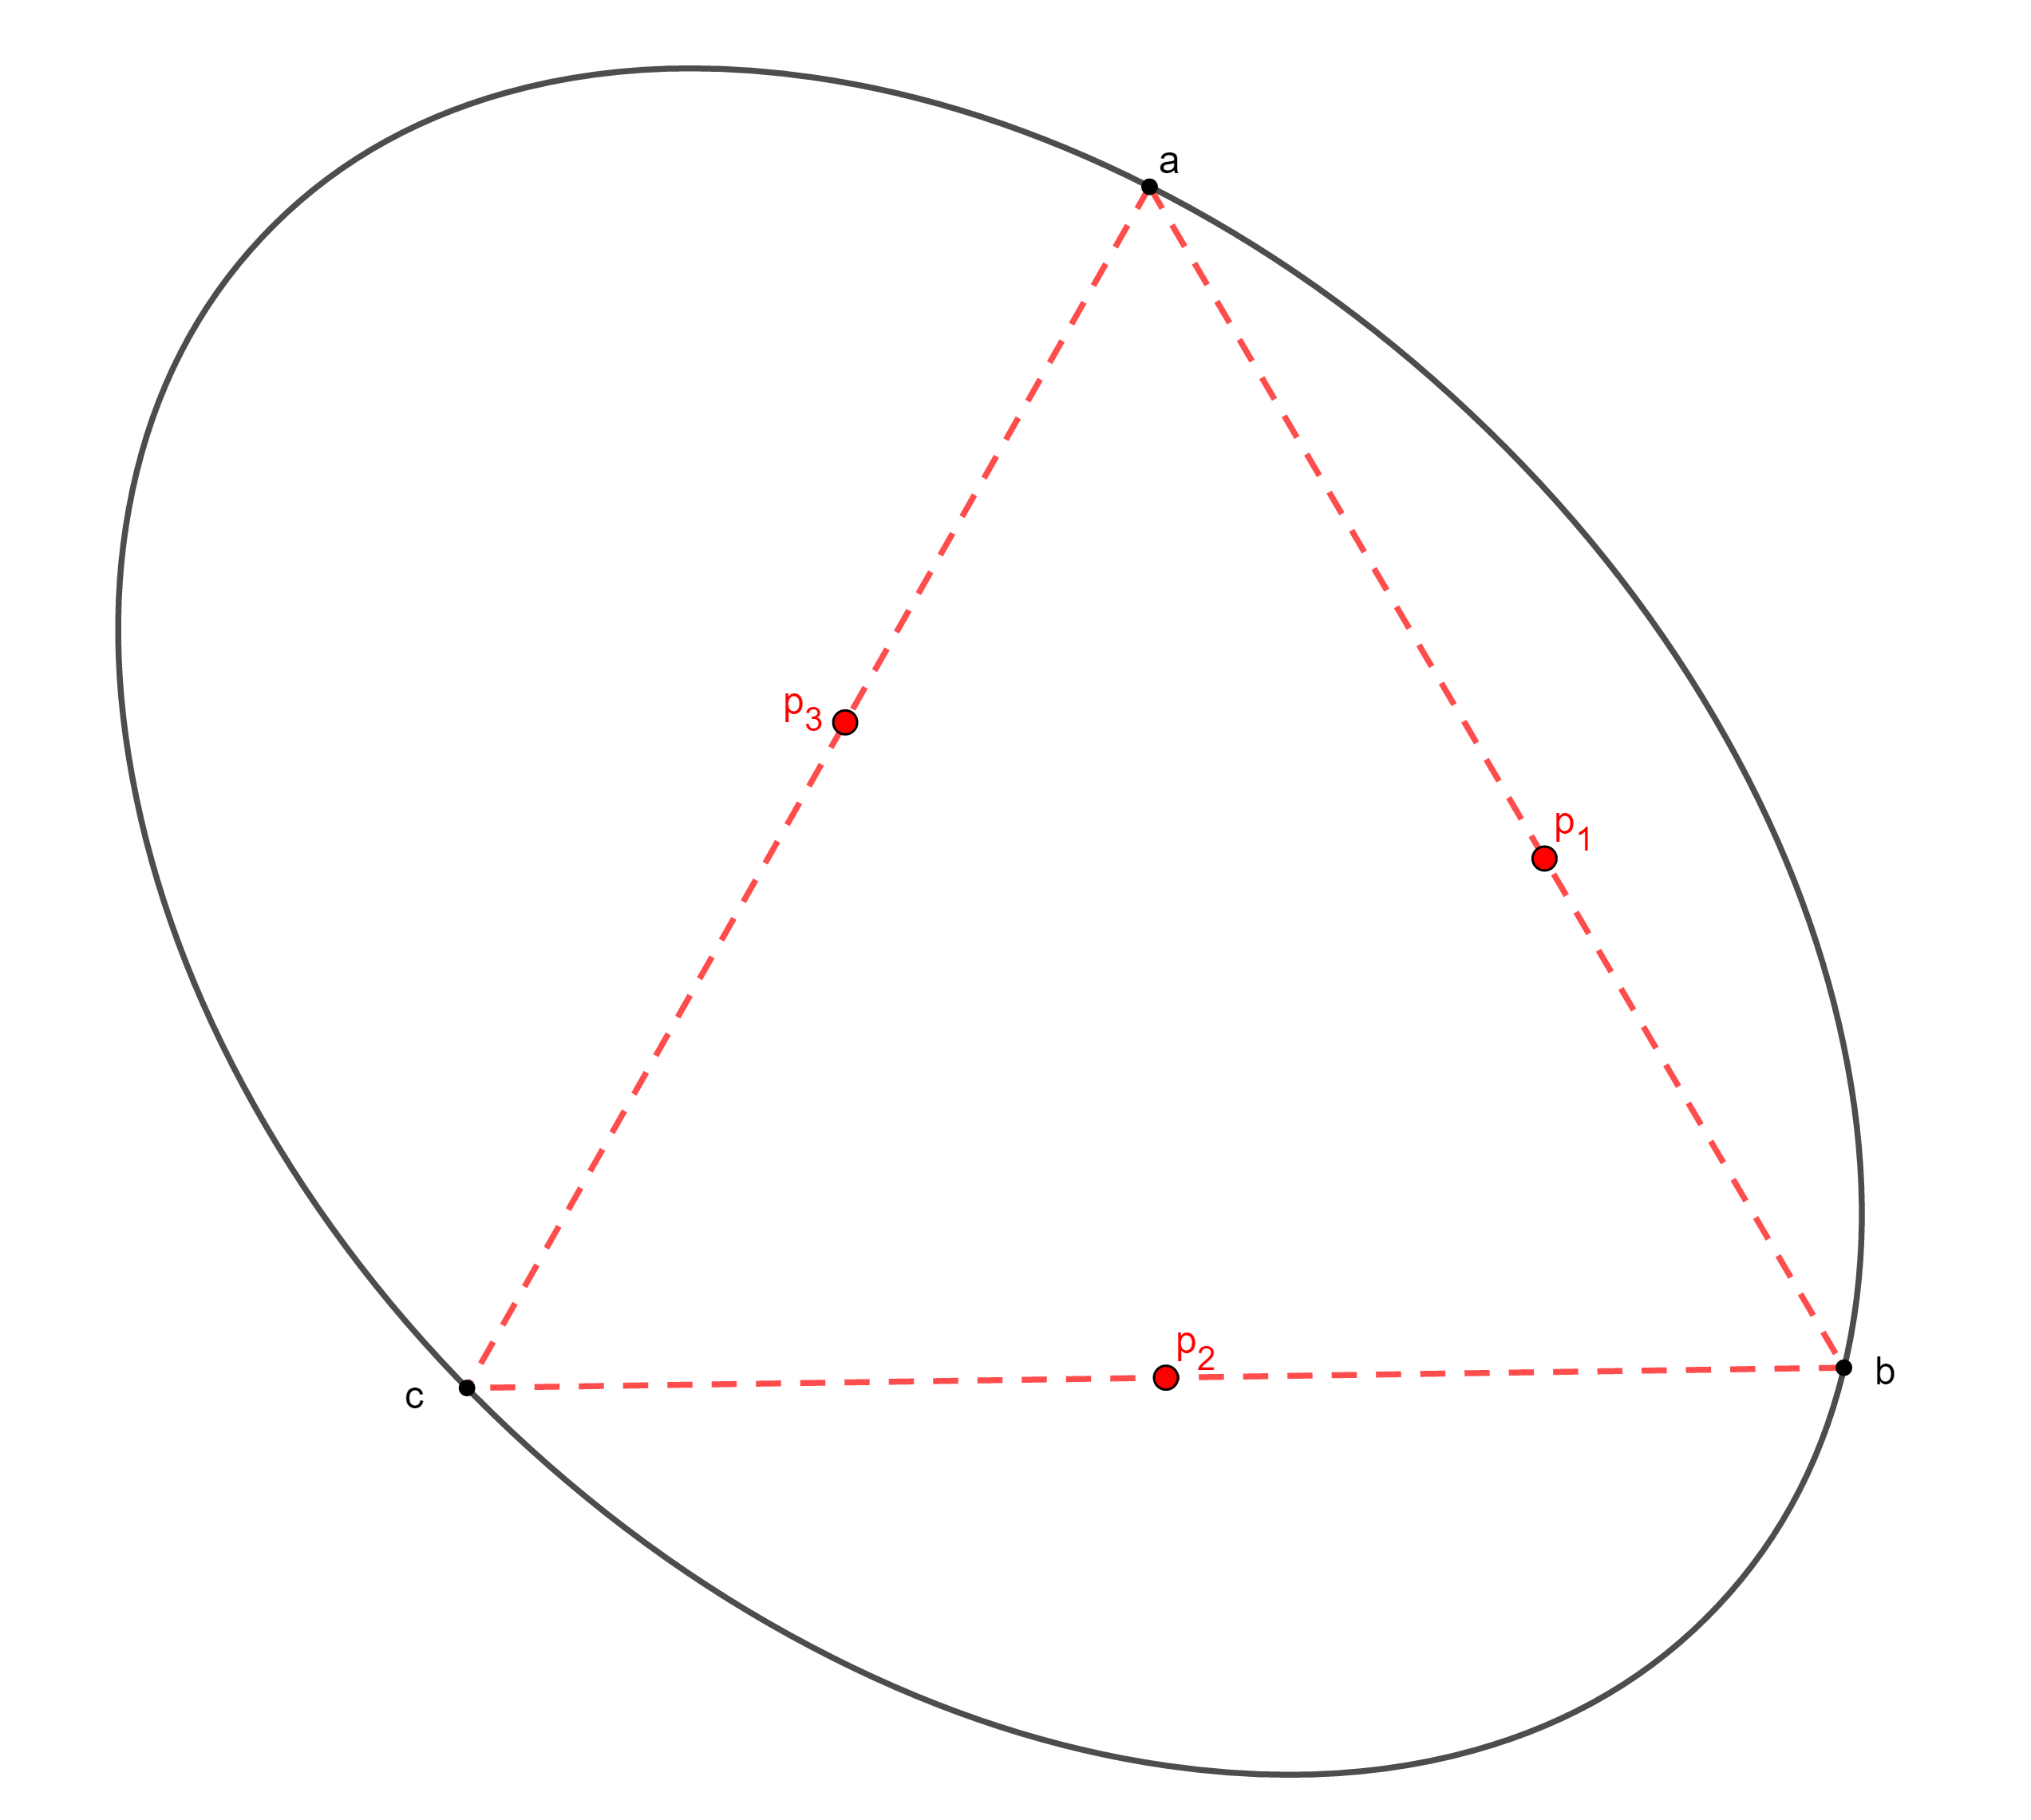
\includegraphics[width=0.35\linewidth]{pic15}
	\end{figure}
	\noindent
	Рассмотрим преобразование при котором вершины треугольника переходят в точки $0,1,\infty$. Заметим что $\angle A P B = \frac{\pi}{2}$. Рассмотрим геодезическую проходящую через $R,P$, заметим что $PB$ касается этой геодезической, так как $AP$ -- радиус окружности, частью которой является $RP$, а $AP \perp BP$. Аналогично $AP$ -- касательная для $PS$. Тогда угол между $PS$ и $PR$ равен углу между $AP$ и $BP$, то есть $\angle RPS = \frac{\pi}{4}$ 
	
	\subsection*{Задача 4}
	\begin{figure}[h!]
		\center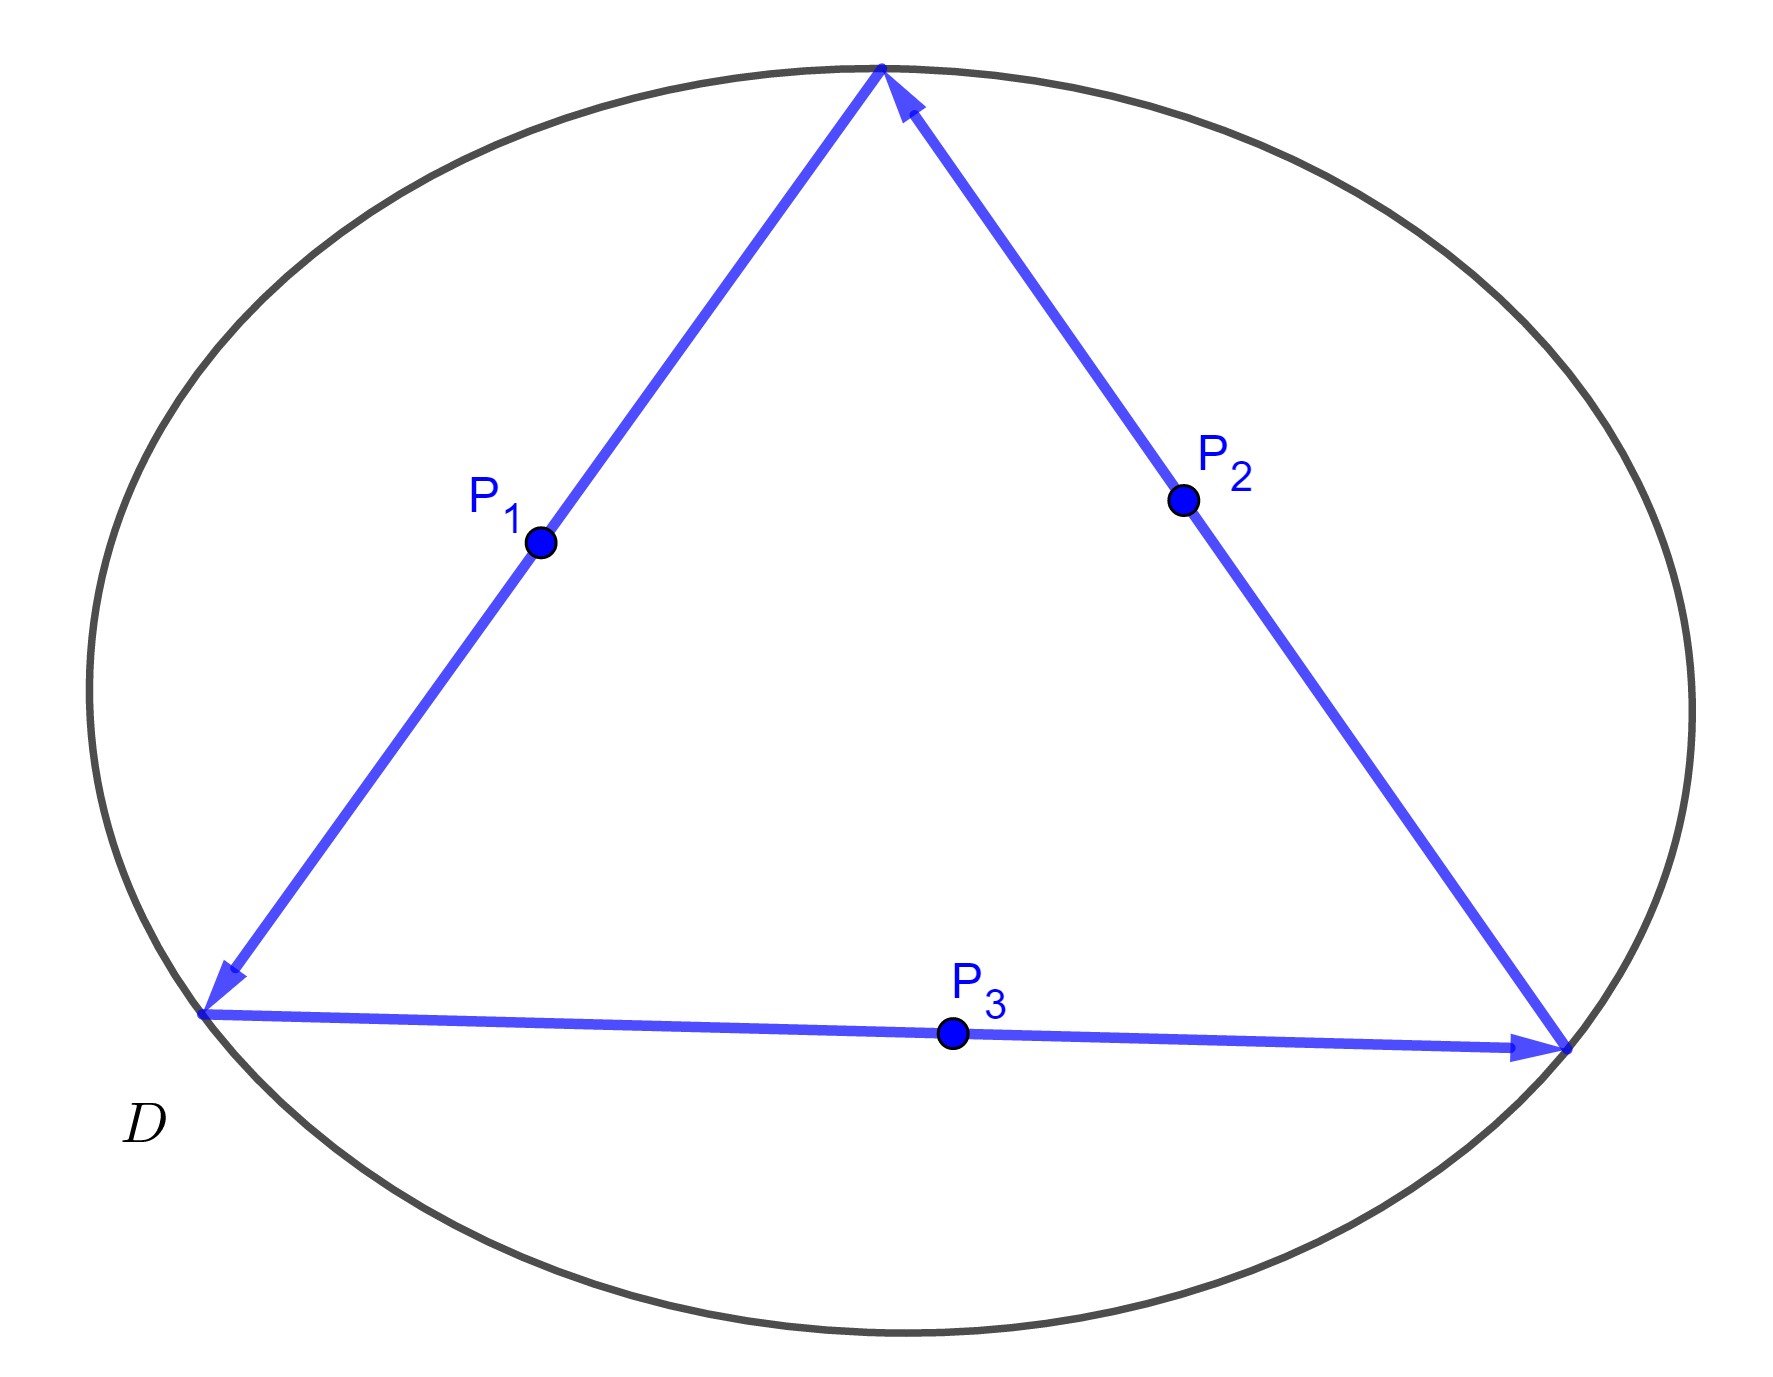
\includegraphics[width=0.5\linewidth]{pic17}
	\end{figure}
	\noindent
	Рассмотрим треугольник в верхней полуплоскости, у которого вершины расположены в точках $0,1,\infty$ и построим орициклы $O_1', O_2'$, проходящие через середину стороны $AB$ и вершины $A,B$. Заметим, что тогда участки $a_1$ и $a_2$ не покрытые $O_1', O_2'$ будут иметь равную длину $l = \frac{a_1 + a_2 - a_3}{2}$. Также $\ln(c_3) = l$, откуда следует $c_3 = e^{-l} = e^{-\frac{a_1 + a_2 - a_3}{2}} = e^{\frac{a_3 - a_1 - a_2}{2}} = \frac{\Lambda_3}{\Lambda_1 \Lambda_2}$, что и требовалось доказать.
	
	\newpage
	\subsection*{Задача 3}
	\begin{figure}[h!]
		\center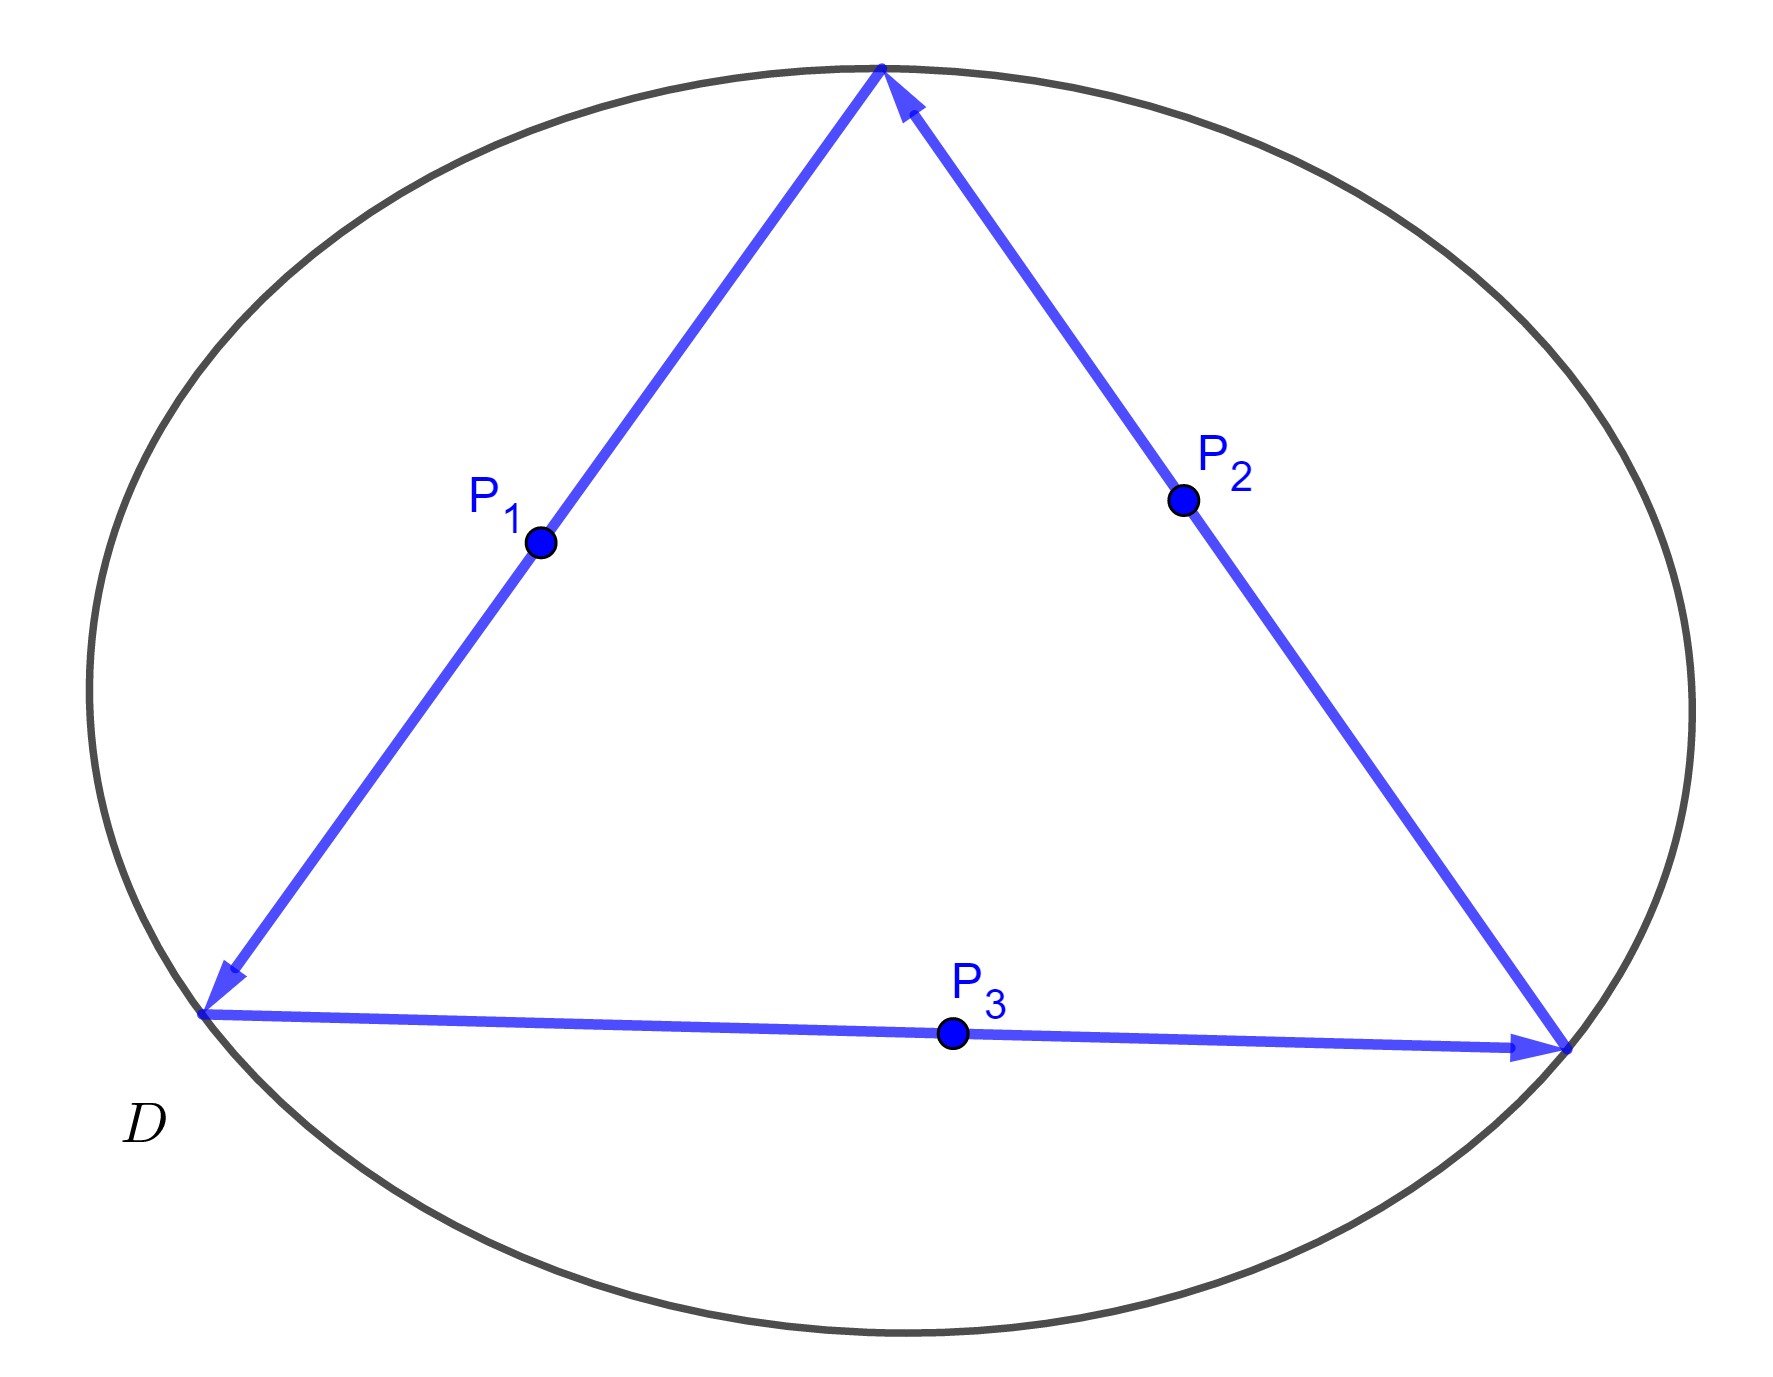
\includegraphics[width=0.5\linewidth]{pic17}
	\end{figure}
	\noindent
	Заметим, что так как $\Gamma_i = e^{\frac{1}{2}a_i}$ то установив биекцию между треугольниками и тройками $(a_i,a_j,a_k)$ мы также установим биекцию между треугольниками и $(\Gamma_i, \Gamma_j,\Gamma_k)$, так как $\Gamma_i = e^{\frac{1}{2}a_i}$ задает биекцию между $(a_i,a_j,a_k)$ и $(\Gamma_i, \Gamma_j,\Gamma_k)$.\\
	Тогда заметим что зная $a_1, a_2, a_3$ можно вывести и $c_1, c_2, c_3$ тем же способом что мы делали и в 4 задаче, тогда мы будем знать все стороны усеченного идеального треугольника, а следовательно однозначно его определим.
	
	
	\subsection*{Задача 5*}
	\begin{figure}[h!]
		\begin{minipage}[h]{0.5\linewidth}
			\center{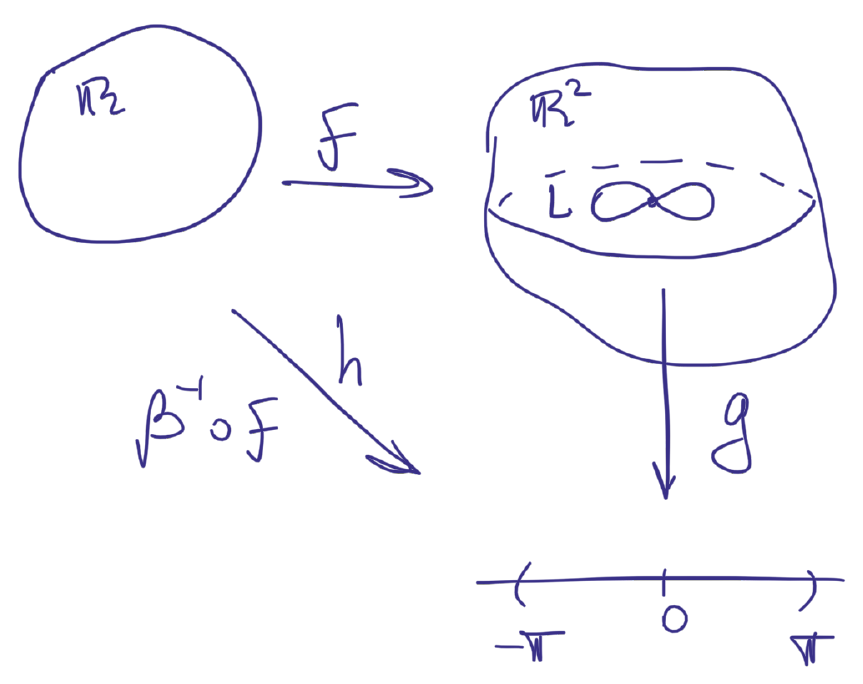
\includegraphics[width=0.8\linewidth]{pic10}}
		\end{minipage}
		\hfill
		\begin{minipage}[h]{0.5\linewidth}
			\center{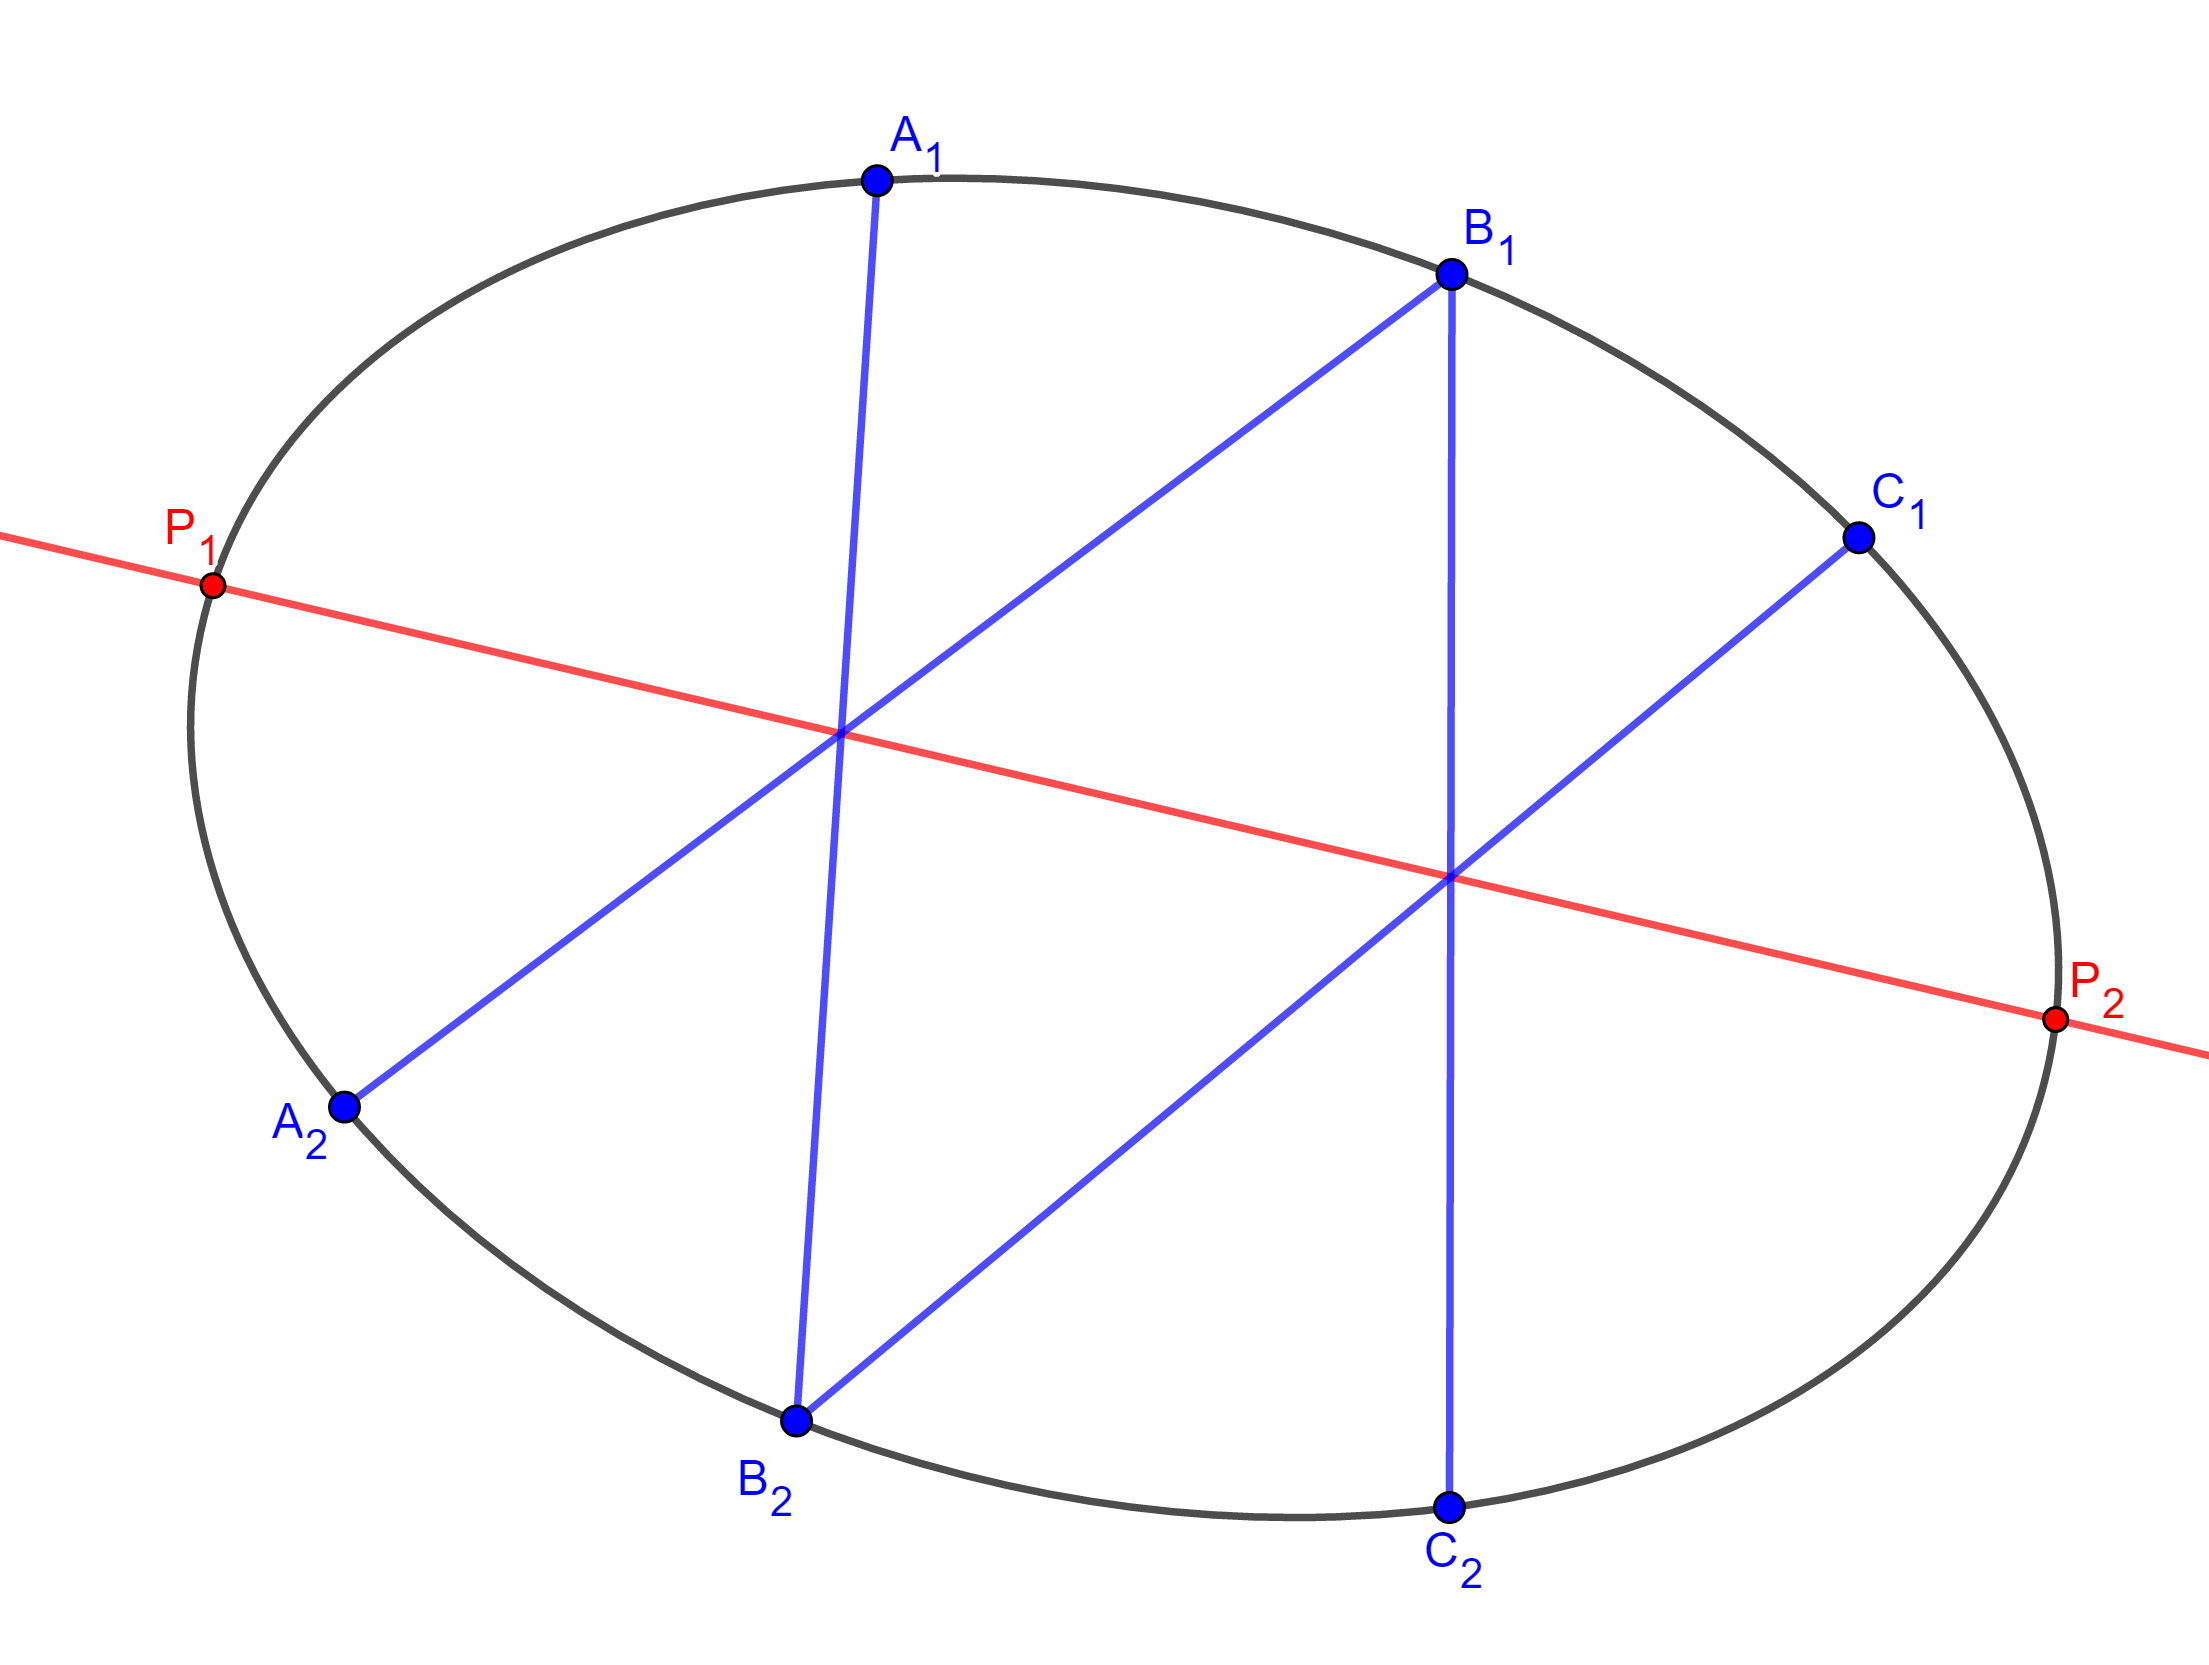
\includegraphics[width=0.8\linewidth]{pic16}}
		\end{minipage}
	\end{figure}
	\noindent
	Рассмотрим один из орициклов, для определенности $O_4$, заметим что для одной из его дуг выполнено 
	\begin{gather*}
		c_{13} = c_{12} + c_{23}
	\end{gather*}
	Тогда, зная что
	\begin{gather*}
		c_{k} = \frac{\Lambda_{k}}{\Lambda_{i} \Lambda_{j}}
	\end{gather*}
	Можно вывести
	\begin{gather*}
		\frac{\Lambda_{13}}{\Lambda_{14} \Lambda_{34}} = \frac{\Lambda_{12}}{\Lambda_{14} \Lambda_{24}} + \frac{\Lambda_{23}}{\Lambda_{24} \Lambda_{34}}
	\end{gather*}
	Домножим на $\Lambda_{14} \Lambda_{24}\Lambda_{34}$
	\begin{gather*}
		\Lambda_{13}\Lambda_{24} = \Lambda_{12}\Lambda_{34} + \Lambda_{23}\Lambda_{14}
	\end{gather*}